\documentclass[10pt, a4paper]{report}
\usepackage[utf8]{inputenc}
\usepackage[T1]{fontenc}
\usepackage[english]{babel}
\usepackage{graphicx}
\usepackage{hyperref}
\usepackage[hypcap]{caption}
\usepackage{listings}
\usepackage{color}
\usepackage[Q=yes]{examplep}

\definecolor{mystringcolor}{RGB}{0,0,0}
\definecolor{mykeywordcolor}{RGB}{127,0,85}
\lstset{
backgroundcolor=\color{white},          % choose the background color; you must add \usepackage{color} or \usepackage{xcolor}
basicstyle=\ttfamily\footnotesize,      % the size of the fonts that are used for the code
breakatwhitespace=false,                % sets if automatic breaks should only happen at whitespace
breaklines=true,                        % sets automatic line breaking
captionpos=b,                           % sets the caption-position to bottom
commentstyle=\color{green},             % comment style
deletekeywords={...},                   % if you want to delete keywords from the given language
escapeinside={\%*}{*)},                 % if you want to add LaTeX within your code
extendedchars=true,                     % lets you use non-ASCII characters; for 8-bits encodings only, does not work with UTF-8
frame=single,                           % adds a frame around the code
keepspaces=true,                        % keeps spaces in text, useful for keeping indentation of code (possibly needs columns=flexible)
keywordstyle=\color{mykeywordcolor},    % keyword style
language=C++,                           % the language of the code
morekeywords={*,...},                   % if you want to add more keywords to the set
numbers=left,                           % where to put the line-numbers; possible values are (none, left, right)
numbersep=8pt,                          % how far the line-numbers are from the code
numberstyle=\footnotesize\color{black}, % the style that is used for the line-numbers
rulecolor=\color{black},                % if not set, the frame-color may be changed on line-breaks within not-black text (e.g. comments (green here))
showspaces=false,                       % show spaces everywhere adding particular underscores; it overrides 'showstringspaces'
showstringspaces=false,                 % underline spaces within strings only
showtabs=false,                         % show tabs within strings adding particular underscores
stepnumber=1,                           % the step between two line-numbers. If it's 1, each line will be numbered
stringstyle=\color{mystringcolor},      % string literal style
tabsize=4,                              % sets default tabsize to 2 spaces
% title=\caption                          % show the filename of files included with \lstinputlisting; also try caption instead of title
}

\begin{document}

\title{Implementing generic multiple precision arithmetic on GPUs}
\author{Alexandre Carlessi \and Sahand Kashani-Akhavan}
\date{\today}
\maketitle

\tableofcontents

\chapter{Introduction}
\section{Background}
For 30 years, one of the primary ways of speeding up electronic devices has been
to increase CPU clock speeds.
From around speeds of 1~MHz in the 1980s, clock speeds have risen to more than
4~GHz in 2013.
Although increasing CPU clock speeds is by far not the \emph{only} way to
increase performance, it has been a reliable source for improvement.
However, fundamental limits in the fabrication of integrated circuits makes it
no longer feasible to just increase clock speeds of existing architectures as a
way to gain more performance.
For years, supercomputers have used another way to increase performance, which
consists of performing more \emph{parallel} work by increasing the \emph{number}
of processors used in machines.

To apply this idea to personal computers, the industry has steadily been
shifting towards multi-core CPUs.
This trend can easily be seen since the introduction of the first dual-core
consumer CPUs in 2005, up to the current high-end 16-core workstation CPUs.
As such, parallel computing is no longer a \emph{niche} that only exotic
supercomputers once claimed to perform.
Indeed, more and more electronic devices have started to incorporate parallel
computing capabilities as an effort to provide functionality well beyond those
of their predecessors.

However, CPUs are not the first devices with parallel computing in mind, as GPUs
have applied this idea earlier.
A graphics processing unit, also known as a GPU, is a specialized electronic
circuit initially designed for fast memory manipulations needed to accelerate
the creation of images in a frame buffer, which are then outputted to a display
for viewing.
Nowadays, GPUs are present in almost all electronics, including, but not limited
to embedded systems, mobile phones, personal computers, workstations, and game
consoles.
Modern GPUs have highly parallel structures, making them much more effective
than general-purpose CPUs for algorithms which process large blocks of data in
parallel.
Thus, GPUs have become very efficient at manipulating imagery, which consists
of applying an algorithm parallely to all output pixels, which explains their
abundant use in computer graphics.

In this report, we explore the implementation of a form of multiple-precision
arithmetic on GPUs in order to leverage their high bandwidth capabilities.

\section{GPU programmability evolution}
GPUs were initially designed to accelerate texture mapping, polygon rendering,
and geometry.
The first GPUs had a fixed-function rendering pipeline, and could not be used
for anything other than common geometry transformations and pixel-shading
functions that were pre-defined in hardware.

With the introduction of the NVIDA GeForce 3 in 2001, GPUs added programmable
shading to their capabilities, which allowed developers to define their own
straight-line shading programs to perform custom effects on the GPU.
Bypassing the fixed-function rendering pipeline opened the door towards many
future graphics novelties, such as cel shading, mip mapping, shadow volumes,
oversampling, interpolation, bump mapping, and many others.

The 2 main shaders were the fragment shader (also known under the name of pixel
shader), and the vertex shader (also known under then name of geometry shader).
The vertex shader processed each geometric vertex of a scene and could
manipulate their position and texture coordinates, but could not create any new
vertices.
The vertex shader's output was sent to the fragment shader for further
processing.
The fragment shader processed each pixel and computed its final color, as well
as other per-pixel attributes by using supplied textures as inputs.
Soon, shaders could execute code loops and lengthy floating point math instead
of straight-line code, which pushed them to quickly become as flexible as CPUs,
while being orders of magnitude faster for image processing operations.
The shaders were written to apply transformations to a large set of elements
parallely, such as to each pixel of the screen, or to every vertex of a 3D
geometric model.

GPUs had different processing units for each type of shader, but with its
introduction in 2006, the NVIDIA~GeForce~8800~GTX merged the separate
programmable graphics stages to an array of unified processors, which allowed
dynamic partitioning of the computing elements to the different shaders, thus
attaining better load balancing.

The unified processor array of the GeForce~8800~GTX is shown on
Figure~\ref{fig:unified_programmable_processor_array_of_the_GeForce_8800_GTX_graphics_pipeline}.
This unified design made GPUs architecturally closer to CPUs.

\begin{figure}[h]
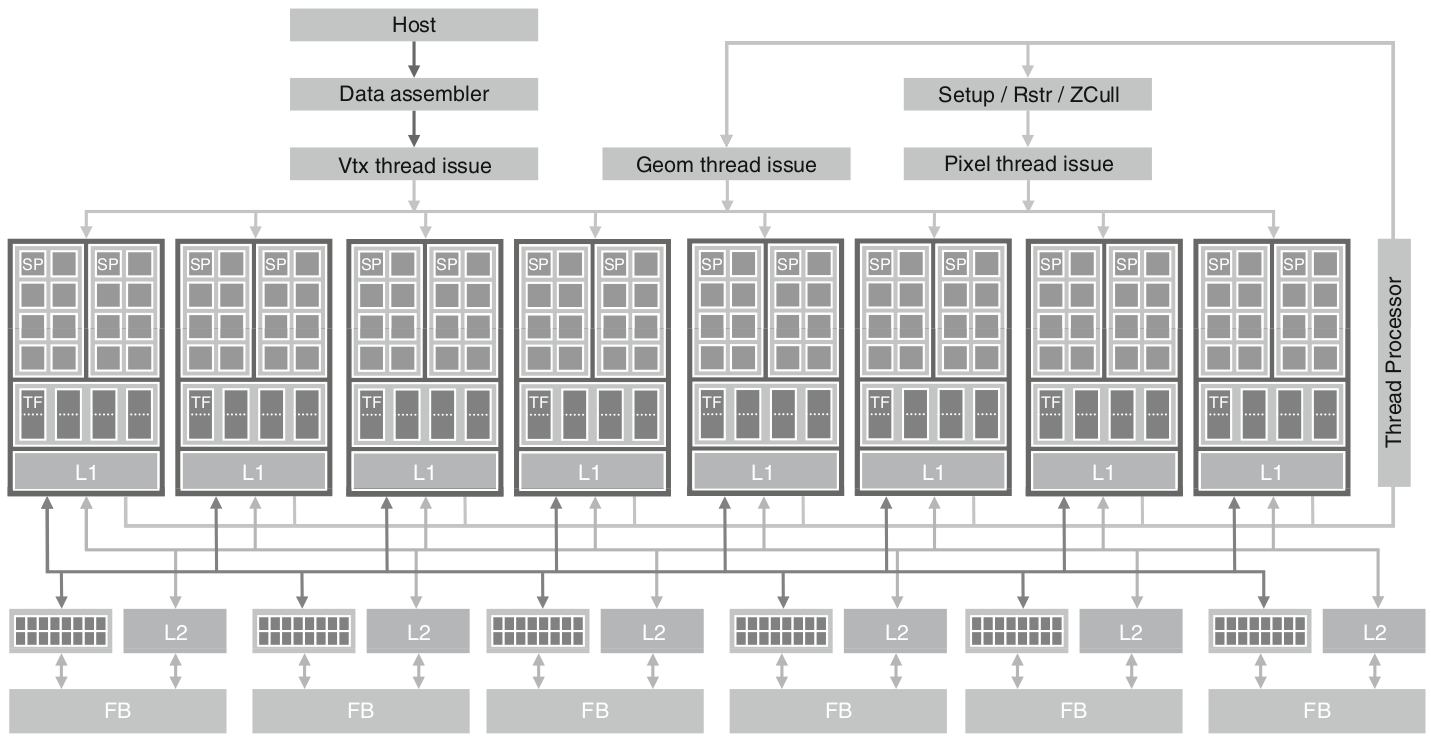
\includegraphics[width=\linewidth]{figs/unified_programmable_processor_array_of_the_GeForce_8800_GTX_graphics_pipeline}
\caption{Unified programmable processor array of the GeForce 8800 GTX}
\label{fig:unified_programmable_processor_array_of_the_GeForce_8800_GTX_graphics_pipeline}
\end{figure}

\section{Early GPGPU}
\subsection{Introduction}
GPU hardware designs evolved towards more unified processors, and were getting
more similar to high-performance parallel computers.
Computations performed by programmable shaders mostly involved matrix and vector
operations, for which GPUs were very well suited (processing blocks of data in
parallel).
The availability of high speed linear algebraic operations, as well as the
unified procesors pushed scientists to start studying the use of GPUs for
non-graphical calculations.
This was achieved through the use of GPGPU techniques.

GPGPU, a shorthand for General Purpose computing on Graphics Processing Units,
consists of using a GPU, which typically only handles computations related to
computer graphics, to perform computations for applications which are
traditionally handled by a CPU.
Such a consideration is possible since GPUs support a functionally complete set
of operations on arbitrary bits, and can thus compute any value.

At the time, programmers could only interface with GPUs through graphics APIs
such as OpenGL or DirectX.
However, APIs had been designed to only support features required in graphics.
To access the GPU's computational resources, programmers had to map their
problem into graphics operations so the computations could be launched through
OpenGL or DirectX API calls.
With this consideration in mind, programmers had to arrange their data in such a
way to ``trick'' the GPU in performing the calculations defined in the
programmers' shaders as if they were graphics calculations, whereas in reality,
they were scientific computations.

\subsection{GPGPU concepts}
There are 4 main GPGPU concepts.

\begin{enumerate}
\item Data arrays are equivalent to GPU textures.
The native data layout for CPUs is the one-dimensional array.
Higher dimensional arrays are available for programmer convenience, but are
actually implemented as one-dimensional arrays, and compilers use linear
transformations to adapt the indices accordingly.

On the other hand, GPUs use two-dimensional arrays as their native data layout
and are, in fact, textures.
To make a data array available to the GPU, the CPU would need to create the
data, then map it to a GPU texture which a shader could later read and process.
In order to correctly use the memory available to a GPU, one needs to find a
mapping between the CPU array indices, and the GPU texture coordinates.
Once the mapping is done, the CPU would then transfer the data towards the GPU
texture.

\item Computation code, also called a \emph{kernel}, is equivalent to a shader.
There is a fundamental difference between the computing model of CPUs and GPUs,
and this impacts the way one needs to think algorithmically.
GPUs follow the data-parallel programming paradigm, whereas CPUs follow the
sequential programming paradigm.

As such, CPU code is usually implemented as a loop-oriented program, since it
has to iterate over all elements of a data structure, and apply a function to
each one.
In contrast, GPUs have highly parallel structures which can apply the same code
to large blocks of data parallely, assuming that there is no dependency among
the operations.

To show the contrast in the programming model, let's compare how one would
compute the addition of 2 $N$-element vectors and store the result in the first
vector.

Assume we have the following 2 vectors already pre-filled with their respective
data:

\lstset{caption={Vector definitions}}
\begin{lstlisting}
  int a[N];
  int b[N];
\end{lstlisting}

The CPU code to perform this vector addition would look like this:

\lstset{caption={Vector addition}}
\begin{lstlisting}
  for (int i = 0; i < N; i += 1)
  {
      a[i] = a[i] + b[i];
  }
\end{lstlisting}

Note that the CPU will have to loop over all indices of the 2 arrays, and add
each element one by one in a sequential way.
It is important to note that each of the $N$ computations are completely
independent, as there are no data dependencies between elements in the result
vector.
For example, once we have computed \verb!a[0] = a[0] + b[0]!, its result will be
of no help when it comes to computing \verb!a[1] = a[1] + b[1]!.

As such, assuming we have a computation unit with $N$ parallel structures, we
could be able to compute the vector addition without the need of any loop by
assigning one vector element addition to each computation unit.
This is easily done by adapting the index of the vector elements that are
provided to each computation unit.

This is the core idea behind GPGPU computing: separating the identical, but
independent calculations from one another, and assigning them to different
execution units which can then execute them at the same time.
Algorithms are extracted into computational kernels which are no longer vector
expressions, but scalar templates of the algorithm that form a single output
value from a set of input values.
These algorithms are implemented in shaders which will then calculate the
independent computations parallely.

For the vector addition used above, the 2 vectors will have to be written into
textures by the CPU, then the shader will read the appropriate elements from the
texture to perform its independent computation.

\item Computations are equivalent to ``drawing''.
Indeed, the final output of a GPU is an ``image'', therefore all computations
have to, in some way or another, write their ``results'' to the frame buffer for
it to be available to the programmer.

The programmer must tell the graphics API (either OpenGL or DirectX) to draw a
rectangle over the whole screen, so that the fragment shader can apply its code
to each pixel independently and output an answer.
If the API were not instructed to draw something that fills the whole screen,
then the fragment shader's code would not be applied to all the data in the
textures we created, but only to a subset of it.

By rendering the simple rectangle, we can be sure that the kernel is executed
for each data item in the original texture.

\item On CPUs, data is read from memory locations, and results are written to
memory locations.
On GPUs, we just saw that the final output is written to the frame buffer.

However, a huge number of algorithms are not straight-line code, and require the
GPU's result to be used as input for another subsequent computation.
To achieve this on a GPU, we need to execute another rendering pass.
This is achieved by writing the current result to another texture, binding this
texture as well as other input or output textures, and potentially also binding
another shader for the algorithm to continue.
This is known as the ping-pong technique since one has to keep juggling between
textures until the algorithm is done and the result is outputted to the frame
buffer.

\end{enumerate}

To recap all that is needed for GPGPU on graphics APIs, one needs to create data
on the CPU, map it to GPU textures, write shaders to perform computations based
on the data in the textures, and finally write the result back to the frame
buffer.

Early GPGPU programming can quickly become quite tedious, even for simple
algorithms, as one must understand the complete graphics rendering pipeline in
order to trick the GPU in thinking it's performing graphics calculations,
whereas the programmers are actually manipulating their data on GPU textures,
and writing their kernels in shaders.

Indeed, graphics APIs were not intended for scientific computations, and are
thus not easily programmable.
In order to fully benefit from the parallel processing power of GPUs without
having to know anything about the graphics rendering pipeline, more
computational oriented languages were created.

\chapter{NVIDIA CUDA}
The Compute Unified Device Architecture, more commonly known under the name
CUDA, is a parallel computing platform and programming model developed by
NVIDIA in 2006, and implemented by the GPUs they produce.

CUDA was designed for GPGPU programming, as developers can compile C code for
CUDA capable GPUs, thus avoiding the tedious work of mapping their algorithms to
graphics concepts.
Essentially, CUDA's main advantage is that developers have explicit access to
the GPU's virtual instruction set, as well as its device memory.
By using CUDA, developers can use GPUs in a similar way as CPUs, without having
to know anything about the graphics rendering pipeline.

CUDA also exposes several GPU hardware features that are not accessible through
graphics APIs, the most important of which is access to GPU shared memory, an
area of on-chip GPU memory which can be accessed in parallel by several blocks
of threads.
CUDA also supports a thread synchronization primitive, allowing cooperative
parallel processing of on-chip data, greatly reducing the high-latency off-chip
bandwidth requirements of many parallel algorithms.

\section{CUDA Program Structure}
A CUDA program consists of multiple interleavings of CPU code segments,
and GPU code segments.
CPU code is called \emph{host} code, whereas GPU code is called \emph{device}
code.
The segments that exhibit little data parallelism are implemented as host code,
whereas the data parallel segments are implemented as device code.

\begin{figure}[h]
\centering
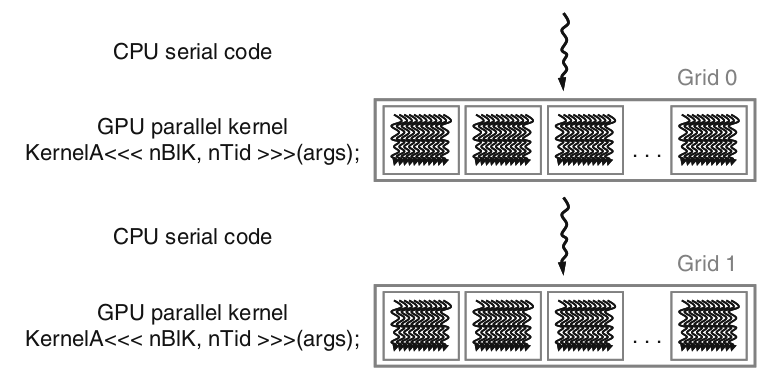
\includegraphics[scale=0.35]{figs/cuda_program_execution_phases}
\caption{Cuda program execution phases}
\label{fig:cuda_program_execution_phases}
\end{figure}

All the code is written in ANSI C extended with keywords for labeling data-
parallel functions called \emph{kernels}, and their associated data structures.
The compilation process separates the host code from the device code, passing
the host code to the host's standard C compiler, and the device code to the
NVIDIA C compiler (nvcc).

In CUDA, computations are carried out by \emph{threads}, a large number of which
are generated by kernels to exploit data parallelism.
Kernels specify the code to be executed by \emph{all} threads during a parallel
segment.
Since all threads execute the same code, the CUDA programming model follows the
\emph{SIMT} (Single Instruction Multiple Thread) programming style.
A representation of the CUDA program execution flow is shown in
Figure~\ref{fig:cuda_program_execution_phases}.

\section{CUDA thread organization}
\label{sec:cuda_thread_organization}
When a kernel is launched, a \emph{grid} of parallel threads are executed.
Threads in a grid are organized into a two-level hierarchy, as shown in
Figure~\ref{fig:cuda_thread_organization}.
A grid consists of one or more thread blocks, each of which contain the same
number of threads.
Each thread block has a unique 1D, 2D, or 3D block identifier (note that for
simplicity, a 2D identifier is drawn in
Figure~\ref{fig:cuda_thread_organization}).
Similarly, each thread within a block has a unique 1D, 2D, or 3D thread
identifier.

\begin{figure}[h]
\centering
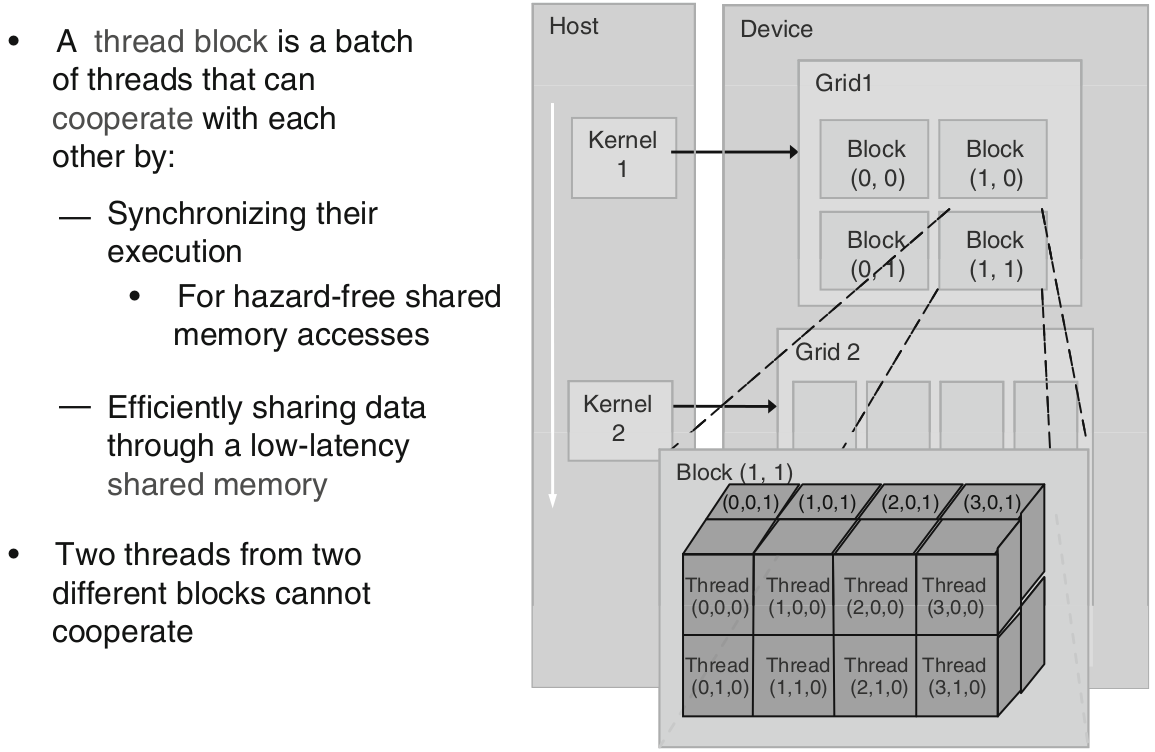
\includegraphics[scale=0.27]{figs/cuda_thread_organization}
\caption{Two-level CUDA thread organization}
\label{fig:cuda_thread_organization}
\end{figure}

Once a kernel is launched, the CUDA runtime generates the corresponding grid of
threads, which are then assigned to execution resources on a block-by-block
basis.
To have some numbers, NVIDIA's Fermi (compute capability 2.0) and Kepler
(compute capability 3.0) architectures can have a maximum of 1024 threads
concurrently running in a block.

CUDA execution resources are organized into streaming multiprocessors (SMs), two
of which are shown in Figure~\ref{fig:sm_thread_block_assignment}.
A maximum number of blocks can be assigned to each SM (8 on Fermi GPUs, and 16
on Kepler GPUs) as long as there are enough resources to satisfy the needs of
all the blocks.
If any of the resources needed for the simultaneous execution of the blocks are
unavailable, less blocks will be scheduled for execution on the SM.
The remaining blocks will execute once the resources needed are available again.

\begin{figure}[h]
\centering
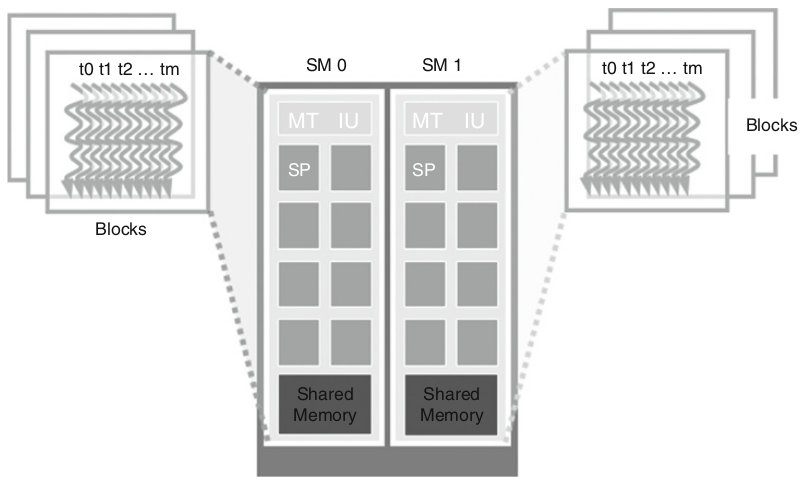
\includegraphics[scale=0.4]{figs/sm_thread_block_assignment}
\caption{SM thread block assignment}
\label{fig:sm_thread_block_assignment}
\end{figure}

Although blocks are scheduled to be run on an SM, it is the threads of that
block that execute the computations.
All threads of a block are scheduled for execution in structures called warps,
each of which contain 32 continuous threads (identified by their $threadIdx$
values).

A crucial aspect about warps is that the hardware executes an instruction for
all threads in the same warp \emph{before} moving to the next instruction.
This works well when all threads within a warp follow the same control flow path
when working on their data.
For example, \emph{if-then-else} style branch statements work well when either
all threads take the \emph{then} statement, or all the threads take the
\emph{else} statement.
If some threads execute the \emph{then} part, and others execute the \emph{else}
part, the SIMT execution model no longer works and the warp will require
multiple execution passes through the divergent paths, with one pass for each
divergent path.
These passes occur sequentially, thus increasing the execution time.
The situation is even worse for \emph{while} loops, since the each thread could
potentially loop a different number of times compared to the others, therefore
it is very important to try and keep thread divergence low.

\section{CUDA memory structure}
In CUDA, the host and devices have separate memory spaces, as GPUs are typically
hardware cards that come with their own DRAM.
In order to provide data to a kernel, memory needs to be allocated on the
device, and data has to be transferred to the allocated memory.
Similarly, after kernel completion, device results must be transferred back from
device memory to host memory.
CUDA devices expose several different memories to developers, some of which are
shown on Figure~\ref{fig:cuda_memory_hierarchy}.
Note that for simplicity, texture memory is not shown.

\begin{figure}[h]
\centering
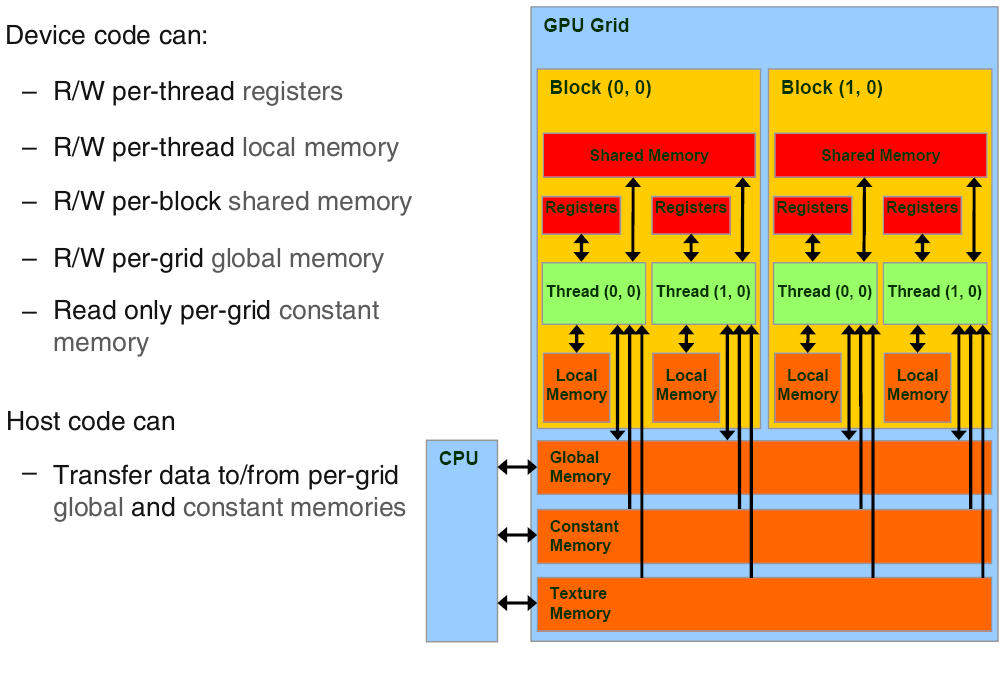
\includegraphics[scale=0.25]{figs/cuda_memory_hierarchy}
\caption{CUDA memory hierarchy}
\label{fig:cuda_memory_hierarchy}
\end{figure}

At the bottom of the figure, we see \emph{global} memory, and \emph{constant}
memory, the 2 off-chip memories available on a CUDA GPU.
Global memory, typically implemented as DRAM, can be written to, and read from
the host.
Because of its implementation technology, global memory suffers from long access
latencies, and finite access bandwidth.
In contrast, constant memory supports short-latency, high-bandwidth, read-only
access by the device when all threads simultaneously access the same location.
Registers and shared memory are on-chip memories, and are thus accessible at
very high speeds, and in a parallel way.

\section{Maximizing global memory bandwidth}
Because of DRAM's high access latency, global memory is organized in such a way
that when reading a certain location, several consecutive memory locations are
returned.
As such, if an application can make use of multiple consecutive global memory locations
before moving to other locations, the DRAMs can supply the data at a much higher
rate than if random locations are accessed.

When all threads in a warp execute a load instruction, the hardware detects if
the threads are accessing consecutive global memory locations, and if it is the
case, then it does not issue multiple separate load instructions, but will
combine, or \emph{coalesce} them into less load instructions.
To achieve anywhere close to the peak advertised global memory bandwidth, it is
important to take advantage of global memory coalescing, by organizing data in
memory in such a way that each thread can read the data it needs at the same
time as the other threads without requiring separate loads.

\subsection{Example}
Suppose 4 threads are trying to read a \verb+4x4+ matrix \verb+m[4][4]+:

\begin{figure}[h]
\centering
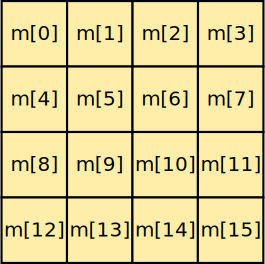
\includegraphics[scale=0.50]{figs/4x4_matrix}
\label{fig:4x4_matrix}
\end{figure}

\hspace{0pt} \\ \\
Normal CPU code for accessing such a matrix would ressemble the following:
\lstset{caption={Accessing matrix elements on a CPU}}
\begin{lstlisting}
  for (int i = 0; i < 4; i++)
  {
      for (int j = 0; j < 4; j++)
      {
          m[i][j] = ... ;
      }
  }
\end{lstlisting}

\hspace{0pt} \\
If we use 4 GPU threads, we get the following code:

\lstset{caption={Accessing matrix elements on a GPU (non-coalesced version)}}
\begin{lstlisting}
  for (int j = 0; j < 4; j++)
  {
      m[threadIdx.x][j] = ... ;
  }
\end{lstlisting}

\hspace{0pt} \\
This matrix is stored in memory as a continuous 1D array of data, and accessing
the data on the GPU with 4 threads parallely would look like this (first loop
iteration):

\begin{figure}[h]
\centering
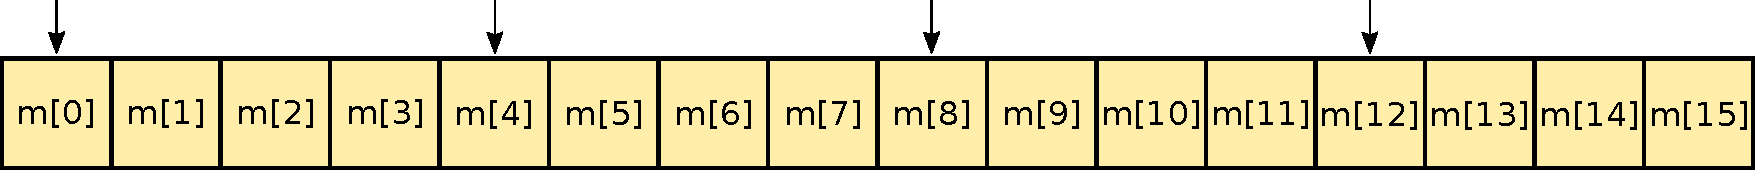
\includegraphics[width=\linewidth]{figs/4x4_matrix_non_coalesced_memory_access}
\caption{Non-coalesced memory access}
\label{fig:4x4_matrix_non_coalesced_memory_access}
\end{figure}

\hspace{0pt} \\
Note that each thread tries to load its ``line'' at the same time as the others,
resulting in 4 scattered global memory reads.
What we would want to have, is reads of the following form:

\begin{figure}[h]
\centering
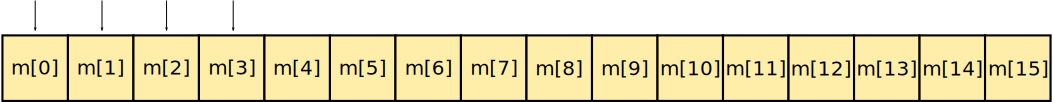
\includegraphics[width=\linewidth]{figs/4x4_matrix_coalesced_memory_access_no_transpose}
\caption{Coalesced memory access}
\label{fig:4x4_matrix_coalesced_memory_access_no_transpose}
\end{figure}

\hspace{0pt} \\
The code corresponding to the memory access pattern in
Figure~\ref{fig:4x4_matrix_coalesced_memory_access_no_transpose} is:

\lstset{caption={Accessing matrix elements on a GPU (coalesced version)}}
\begin{lstlisting}
  for (int j = 0; j < 4; j++)
  {
      matrix[j][threadIdx.x] = ... ;
  }
\end{lstlisting}

\hspace{0pt} \\
But then, each thread would no longer be accessing the element it initially
wanted, as all threads in
Figure~\ref{fig:4x4_matrix_coalesced_memory_access_no_transpose} are accessing
thread 1's ``line''.
The solution to this problem is to transpose the initial matrix, thus yielding
the correct memory access pattern, as well as the minimum number of global
memory accesses:

\begin{figure}[h]
\centering
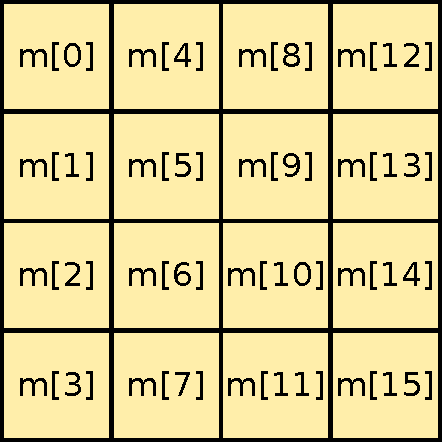
\includegraphics[scale=0.50]{figs/4x4_matrix_transposed}
\caption{Transposed matrix}
\label{fig:4x4_matrix_transposed}
\end{figure}

\begin{figure}[h]
\centering
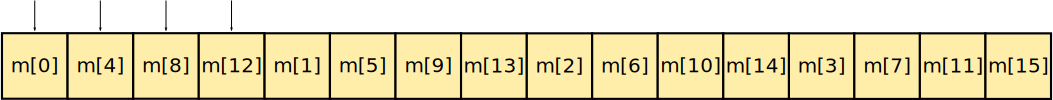
\includegraphics[width=\linewidth]{figs/4x4_matrix_coalesced_memory_access}
\caption{Correct coalesced memory access}
\label{fig:4x4_matrix_coalesced_memory_access}
\end{figure}

\hspace{0pt} \\
Therefore, a ``simple'' port of CPU code is to transpose data arrays, since
concurrent GPU threads can load columns more efficiently.
One must strive for perfect per-warp memory coalescing by aligning starting
addresses (may need padding for this), and accessing continuous memory regions,
all in order to reduce global memory accesses, and to maximize bandwidth.

\section{Performance summary}

So, in order to make sure to take the most advantage of execution units, the
following properties must hold:

\begin{enumerate}
\item Make sure \emph{all} global memory reads and writes are coalesced whenever
possible.
If memory coalescing is not done, then all other so called ``optimizations''
would mostly be insignificant.
In case global memory accesses are difficult to coalesce, it is better to try
and use 1D texture lookups instead, as they are more suited for scattered access
patters.
\item If any data is to be common between threads, do not use global memory with
locks, but rather try to use shared memory as much as possible, since it is much
faster.
\item Minimize the use of all divergent branches, or at least make them the
shortest possible.
\end{enumerate}

\chapter{Implementation}
\section{Data representation}
\subsection{CPU vs GPU representations}
Nowadays, fields such as cryptography, require the ability to perform
computations on very large integers.
In C, multiple precision arithmetic is not built into the language, therefore
one must use external libraries to have the feature.
Until now, one of the reference libraries has been the GNU Multiple Precision
Arithmetic Library, more commonly called GMP.
GMP is a free library for arbitrary precision arithmetic, operating on signed
integers, rational numbers, and floating point numbers.
There is no practical limit to the precision except the ones implied by the
available memory in the machine GMP runs on.
GMP is a reference, because it is carefully designed to be as fast as possible,
both for small operands, and for big operands by using fullwords as the basic
arithmetic type, fast algorithms, and highly optimized assembly code.

GMP keeps integers in a structure called \verb+mpz_t+.
Each \verb+mpz_t+ structure stores numbers under sign and magnitude
representation, which involves keeping the number's sign bit in a field,
separate from its absolute value, which is contained in another field.
The number's absolute value is represented as an array of unsigned integers.
Each \verb+mpz_t+ may be composed of a different number of machine words, in
order to maintain maximum memory efficiency.

It is important to note that while GMP uses \emph{sign and magnitude}
representation for its integers, native machine integers are stored in another
form called \emph{two's complement} representation.
Two's complement notation has many advantages at the hardware level, but its
main drawback is that it is bit-length dependent, and is thus impossible
to use for multiple precision arithmetic, for which one does not know in advance
what the precision of its operands are going to be.

By examining the source code of some operations over \verb+mpz_t+, we can easily
see that its efficiency comes from its ability to take care of all ``corner
cases'' appropriately.
This is done by using a huge number of branches in order to steer the execution
towards the most efficient way to perform the computation.
For example, let's briefly examine the GMP multiplication code.
The GMP multiplication code performs the following:

\begin{enumerate}
\item Checks if one operand is bigger than the other, switching operand pointers
and sizes if it is the case.
\item Checks if native long multiplication is supported by the processor.
\item Checks if the bigger operand is less than 2 machine words, in which case
it decides to perform the ``naive'' schoolbook multiplication instead of
asymptotically better algorithms, such as the Karatsuba-Offman algorithm, or the
Toom-Cook algorithm, since their overhead makes them less efficient at small
operand sizes.
This operation is one machine instruction if the processor supports long
multiplication natively, otherwise multiple instructions are used.
\item If the operands are not bounded by 2 machine words, then further tests are
carried out so as to determine which multiplication algorithm should be used to
compute the result more efficiently.
\item Once the computation is performed, the result is returned.
\end{enumerate}

\hspace{0pt} \\
Of course, several memory management stages are interleaved within the
computations to maintain space efficiency.
Many more tests take place in the code, but the most important ones are listed
above.

GMP has worked well until now, since it has been running on CPUs, which support
very efficient sequential execution pipelines.
However, if we were to use GMP directly on GPUs, program execution speed may be
very disappointing.
In section~\ref{sec:cuda_thread_organization}, we wrote about the SIMT execution
model GPUs employ, and the importance for each thread to execute the same
instruction.
However, as seen previously, GMP code contains deepy nested branches, leading to
high potential for divergent branches during execution.
If one were to launch thousands of threads, each of which executes the GMP code
for multiplication, in which each thread has a potential chance to follow a
divergent branch, then performance would be disappointing.

In order to support efficient arithmetic on GPUs, we need to guarantee that each
thread follows the most divergent-free path possible.
Indeed, GPUs are \emph{throughput}-oriented devices, whereas CPUs are
\emph{latency}-oriented devices.
CPUs can have highly optimized code which can decide how to compute \emph{each}
single instance the most efficiently possible, whereas GPUs must provide more
general algorithms which will compute \emph{all} threads parallely,
independently of the fact that each individual thread \emph{could} have executed
the computation in a more efficient way.
It is a GPU's architecture which defines this behaviour.
Therefore, the main idea to grasp here is that one cannot optimize operations on
a thread-by-thread basis.

\subsection{Our bignum representation}
Our initial project idea was to work towards solving the 131-bit Certicom ECC
challenge.
The challenge is to compute ECC private keys from a given list of ECC public
keys and associated system parameters. This is the type of problem an adversary
would face when attempting to defeat an elliptic curve cryptosystem.

This field uses \emph{fixed}-precision modular arithmetic for computations,
therefore it does not explicitly need dynamic runtime-level multiple precision
arithmetic.
This means that once a specific precision is chosen for the Certicom challenge,
\emph{all} operations will be bounded by a certain size constraint.
For example, supposing we choose to solve the 131-bit Certicom challenge, we
will know in advance that integers are going to be at most 131 bits in length.
With this information, we can implement algorithms which operate on this exact
precision the most efficiently possible.
Even if we were to have to represent a 2-bit integer, we would use 131 bits of
storage in order to make sure the representation is consistent between all
threads.
Note that we only need to be able to represent integers consistently, as
ECC cryptography does not use any floating point values.

Unlike general multiple precision libraries like GMP, we decided not to use a
sign and magnitude representation for our integers, since we have an upper bound
on the precision of our operands.
Thus, we decided to store our numbers in two's complement representation.
The advantage of two's complement representation is that the fundamental
arithmetic operations of addition, subtraction, and multiplication are identical
to those for unsigned binary numbers (as long as the inputs are represented in
the same number of bits).

In order to take the most advantage of a device, it is useful to represent data
in its primary data type, which consists of 32-bit fullwords for CUDA GPUs.
We will store our numbers as arrays of these fullwords, so as to have the most
compact notation possible.
In order to store $X$-bits using 32-bit words, one would need at least
$\lceil \frac{X}{32} \rceil$ words.
For 131-bit numbers, this means we need 5 words to store each number.

Figure~\ref{fig:big_endian_number_representation} shows a possible number
representation for the 131-bit number
\verb+0x00000004 ADBFB00E 372139F3 5E2503DD B65B9045+, assuming it is stored in
an array named \verb+a+.

\begin{figure}[h]
\centering
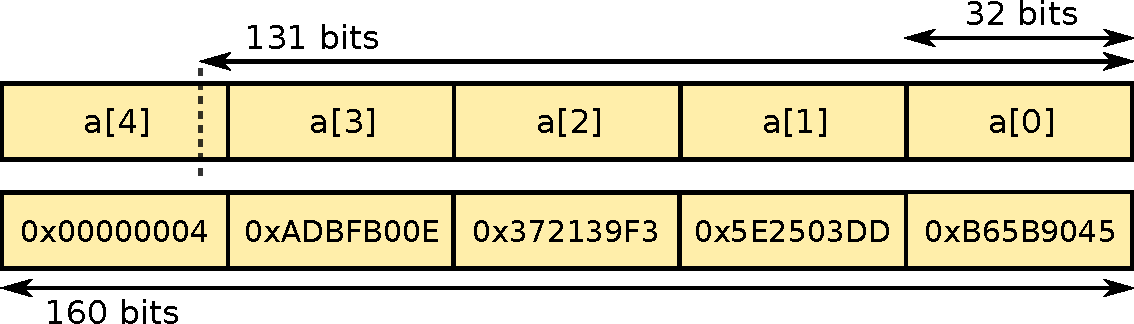
\includegraphics[scale=0.5]{figs/big_endian_number_representation}
\caption{Most significant word first representation (MSW)}
\label{fig:big_endian_number_representation}
\end{figure}

However, for convenience, we decided to store our numbers with their least
significant word first, as all algorithms start from the least significant
words and continue on from there.
This would spare us the need to do constant index manipulations.
Figure~\ref{fig:little_endian_number_representation} shows this alternative
representation.

\begin{figure}[h]
\centering
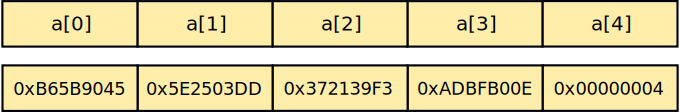
\includegraphics[scale=0.5]{figs/little_endian_number_representation}
\caption{Least significant word first representation (LSW)}
\label{fig:little_endian_number_representation}
\end{figure}

Note that, since we are using two's complement notation, a negative number would
be represented as shown on Figure~\ref{fig:negative_number_representation}, with
several leading \verb+1+s in its MSW.

\begin{figure}[h]
\centering
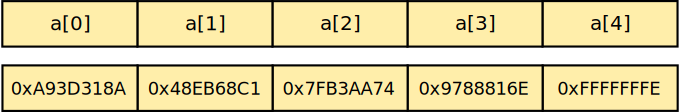
\includegraphics[scale=0.5]{figs/negative_number_representation}
\caption{Negative number representation}
\label{fig:negative_number_representation}
\end{figure}

\section{A note about benchmarks}
In order to benchmark our operations, we prepared different operands, each
containing $1024*1024$ random bignums.
Each operand file was generated for 5 different precisions:

\begin{itemize}
\item 109-bit
\item 131-bit
\item 163-bit
\item 191-bit
\item 239-bit
\end{itemize}

Throughout this document, all benchmarks consist of performing 10 consecutive
executions of each operation.
The amount of random numbers used in the benchmark depends on the total numbers
of threads spawned by the kernel launch configurations, and is equal to
$gridsize*blocksize$.
For example, if we choose to launch a kernel with 1 block and 1 thread, then
only 1 operand will be read from each file, but if we choose to launch a kernel
with 16 blocks and 32 threads, then 512 operands will be read from each file.
We only execute kernels with launch configurations consisting of power of 2
grid sizes and block sizes, so the available launch configurations are
\verb+{1, 2, 4, 16, 32, 64, 128, 256, 512, 1024}+.

We chose this way of benchmarking, because we can set the total amount of
``work'' the GPU must perform, and test what launch configurations work best for
warp occupancy.
For example, suppose we want to test what launch configurations lead to the best
performance for a workload of 64 bignums.
We can try to launch the kernel with the following launch configurations and see
which one gives the best results:

\begin{itemize}
\item 1 block of 64 threads
\item 2 blocks of 32 threads
\item 4 blocks of 16 threads
\item 8 blocks of 8 threads
\item 16 blocks of 4 threads
\item 32 blocks of 2 threads
\item 64 blocks of 1 thread
\end{itemize}

\section{Assembly vs. C}
In order to implement arithmetic over multiple words, one needs be able to
perform carry propagation.
For example, in order to add two 5-word bignums \verb+a+ and \verb+b+, each word
in \verb+a+ must be added to the corresponding word in \verb+b+, yielding a
result, and a potential carry bit.
In turn, this carry bit must be propagated to the next addition involving the
next word of both \verb+a+, and \verb+b+.

We will now describe 2 different ways of accessing the carry bit, and explain
which version we chose to work with, along with the reasons around the decision.

\subsubsection{C}
In C, we do not have access to processor carry flags.
Nevertheless, it is possible to know if a carry was generated by a simple trick.
When a carry flag is generated, it means that the result of an operation is too
big to hold on 32 bits.
This flag can only be generated, if, prior to the operation, there was a binary
\verb+1+ in the leading bit of at least one of the 2 operands, such that the
addition of this leading binary \verb+1+ with a potential other \verb+1+ in the
computation causes the result to overflow.
An illustration is provided in Figure~\ref{fig:addition_overflow_illustration}.

\begin{figure}[h]
\centering
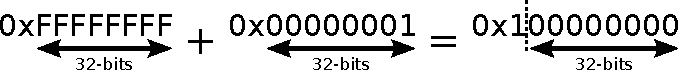
\includegraphics[scale=0.7]{figs/addition_overflow_illustration}
\caption{Overflow on hexadecimal numbers}
\label{fig:addition_overflow_illustration}
\end{figure}

The trick to notice here is that if there was no overflow, then the lower 32
bits of the result would be \emph{bigger or equal} to the lower 32 bits of the
biggest of the 2 operands.
However, if an overflow occurred, then the lower 32 bits of the result is
\emph{smaller} than the lower 32 bits of the the biggest of the 2 operands.
Therefore, in order to get the carry flag for the next computation in C, one
would compute \verb!carry = (c[i] < max(a[i], b[i]))!, then use it for the
\emph{next} addition, like \verb!c[i+1] = a[i+1] + b[i+1] + carry!.
Listing~\ref{lst:N_word_addition_in_C} shows the carry propagation technique for
$N$-word additions.

\lstset{caption={$N$-word addition in C},
        label={lst:N_word_addition_in_C}}
\begin{lstlisting}
c[0] = a[0] + b[0];
for (uint32_t i = 1; i < N; i++)
{
    c[i] = a[i] + b[i] + (c[i-1] < max(a[i-1], b[i-1]));
}
\end{lstlisting}

\subsubsection{Assembly}
CUDA GPUs expose a low-level Parallel Thread Execution (PTX) virtual
machine and instruction set architecture which allows one to program in
pseudo-assembly language.
PTX assembly supports a large set of operations, such as \verb+add+, \verb+sub+,
and \verb+mul+, but in addition, at the time of this writing, it supports 6
extended-precision integer arithmetic instructions (organized into 3
categories), which are listed below.

\begin{enumerate}
\item \verb+add.cc+ (addition with carry-out), \verb+addc+ (addition with
carry-in)
\item \verb+sub.cc+ (subtraction with borrow-out), \verb+subc+ (subtraction with
borrow-in)
\item \verb+mad.cc+ (multiply-add with carry-out), \verb+madc+ (multiply-add
with carry-in)
\end{enumerate}

The special aspect of these instructions is that they reference an implicitly
specified condition code register having a single carry flag bit, which can hold
carry-in, carry-out, borrow-in, or borrow-out flags.
Another important fact is that the condition code is \emph{not} preserved across
calls, and is only intended for use in straight-line code sequences for
computing extended-precision integer addition, subtraction, and multiplication.
PTX can be written in C programs as inline assembly, thus allowing one to write
kernel sections involving normal arithmetic in C, and writing the
extended-precision parts in PTX.

As an example, in order to calculate the extended-precision addition of two
131-bit numbers \verb+a+ and \verb+b+, and store the result in \verb+c+, one
would use the following inline PTX code (remember that \verb+a+, \verb+b+, and
\verb+c+ are 5-word arrays):

\lstset{caption={5-word hand unrolled addition in PTX},
        label={lst:5_word_hand_unrolled_addition_in_PTX}}
\begin{lstlisting}
asm("add.cc.u32  %0, %1, %2;" : "=r"(c[0]) : "r"(a[0]), "r"(b[0]));
asm("addc.cc.u32 %0, %1, %2;" : "=r"(c[1]) : "r"(a[1]), "r"(b[1]));
asm("addc.cc.u32 %0, %1, %2;" : "=r"(c[2]) : "r"(a[2]), "r"(b[2]));
asm("addc.cc.u32 %0, %1, %2;" : "=r"(c[3]) : "r"(a[3]), "r"(b[3]));
asm("addc.u32    %0, %1, %2;" : "=r"(c[4]) : "r"(a[4]), "r"(b[4]));
\end{lstlisting}

In the above addition code, notice that the assembly instructions are identical
for the middle section, as the same operation is taking place.
One would be tempted to write the code in a loop instead, such as the following:

\lstset{caption={5-word loop-oriented addition}, label={}}
\begin{lstlisting}
asm("add.cc.u32  %0, %1, %2;" : "=r"(c[0]) : "r"(a[0]), "r"(b[0]));
for (uint32_t i = 1; i < 4; i++)
{
    asm("addc.cc.u32 %0, %1, %2;" :
        "=r"(c[i]) : "r"(a[i]), "r"(b[i]));
}
asm("addc.u32    %0, %1, %2;" : "=r"(c[4]) : "r"(a[4]), "r"(b[4]));
\end{lstlisting}

The problem with this code is that its result is unpredicatable, since
\emph{carry flags are not preseved across calls}, and the loop structure created
in C around the assembly will \emph{sometimes} make us lose the carry bit.
We initially thought a potential solution to this problem would be to make the
compiler unroll the loop (since we know the number of loop iterations) with the
\verb+#pragma unroll+ directive, as doing so would give us straight-line
assembly code, therefore preseving the carry bit.

\lstset{caption={Compiler unrolled 5-word loop-oriented addition}}
\begin{lstlisting}
asm("add.cc.u32  %0, %1, %2;" : "=r"(c[0]) : "r"(a[0]), "r"(b[0]));
#pragma unroll
for (uint32_t i = 1; i < 4; i++)
{
    asm("addc.cc.u32 %0, %1, %2;" :
        "=r"(c[i]) : "r"(a[i]), "r"(b[i]));
}
asm("addc.u32    %0, %1, %2;" : "=r"(c[4]) : "r"(a[4]), "r"(b[4]));
\end{lstlisting}

However, extensive testing showed that this approach does not guarantee that the
carry is preserved either.
The only solution which works well with inline assembly is that the code be
fully hand-unrolled, such as in
Listing~\ref{lst:5_word_hand_unrolled_addition_in_PTX}.

\subsubsection{Why we chose assembly over C}
\label{sec:why_we_chose_assembly_over_c}
This project was initially about implementing multiple precision arithmetic in
order to be able to implement Pollard's Rho algorithm, and to study the effect
of warp occupation on performance.
Since the arithmetic used in this algorithm consists of modular operations, we
knew in advance that we only needed operations to support a certain precision.
So, the problem is defined as trying to implement operations the most
efficiently possible, by knowing the precision of the operands in advance.
The basic principle we used for our implementation was to make the operations
work for a specific precision, then try to generalize it from there, in order
for it to work on different ones.

At first, we were trying to implement one pure C function per operation.
These functions would take the precisions of their operands as inputs, then
execute the operation to the best they could.
This was easy to do for addition and subtraction, because they use very regular
algorithms and could be implemented by a simple loop along with the carry
propagation trick.

Problems started to arise once we took on the multiplication implementation.
Indeed, for the multiplication to work efficiently, we sometimes needed to test
a condition with respect to the operand precisions, in order to know if some
element even needs to be evaluated.
For example, we know that the multiplication of two $N$-bit numbers can yield a
number of at most $2N$ bits.
One can also generally say that the multiplication of two $k$-word numbers can
yield a number of at most $2k$-words.
However, there are some cases where optimizations could be performed.
For example, 131-bit numbers are representable on 5 words, and their
multiplication could yield numbers of at most $2*131=262$ bits in size.
But, 262-bit numbers can be represented on $\lceil \frac{262}{32} \rceil = 9$
words instead of $5*2=10$ words.
An optimization one could do here is to test if the size of the multiplication
result does need 10 words, and to perform the computation only if necessary.
Since all threads are performing computations on operands of the same precision,
the test will not cause any thread divergence, and all threads would perform the
``optimization''.
However, it is wasteful to perform a test if all threads are going to respond
identically to it, as it becomes equivalent to pure overhead.

What would be best is if one could have precision-specific code at compile time,
so that each thread would only be executing straight-line code, and would not
have any branches to decide upon.
It is possible to do this with the C preprocessor, however there are some
other things we would like to do that are not possible with the preprocessor,
such as code loops \ldots

The solution we came up with was to use a form of metaprogramming by having
pre-compilation scripts which would, in function of the precision provided,
proceed to ``create'' the code for each operation.
The scripts would apply all optimizations needed for the specific precision, and
one would be left with functions which could perform the operations as
straight-line code.

One important note about our scripts is that they do not work for \emph{all}
given precisions.
What we wanted was for the scripts to create functions that will perform
computations for the user as a black box which simply returns the exact answer.
In C, we do not have the guarantee that the result of an addition is exact (it
is possible an overflow will occur), however, our scripts choose to \emph{not}
handle precisions for which unexact answers would be possible by making sure
that \emph{addition} results would \emph{not} need more storage than its
operands.
For example, our script will not work on 128-bit numbers, because the addition
of two 128-bit numbers will potentially give a 129-bit number, which in turn
would require 1 more word to be represented.
Therefore, our scripts will not work for precisions which are multiples of 32.
We took this decision to be sure users could use the same array size to hold
addition or subtraction operands and results, as well as modular addition or
subtraction operands and results.
They would not need to keep track of separate arrays, each of different sizes,
in order for each operation to have enough precision for its result.

Something that was very important for us was that the scripts be the most
generic possible, so others could potentially re-use its output for future
projects, since it is a bit wasteful to have to implement arithmetic again and
again for each new precision one chooses.
One could then focus on their application, instead of the ``basic'' arithmetic,
which turned out to be not so basic in the end.

However, through experimentation, we have to say what C achieves to do better
than our assembly statements.

\begin{itemize}
\item By choosing to use PTX assembly, we have limited ourselves to CUDA-capable
GPUs only, instead of all the AMD GPUs also available.
\item Compiler technology has advanced a lot and it is way ahead of us when it
comes to optimizations, as it can more aggressively tune C code compared to
our assembly, sometimes leading to less register usage.
The performance difference between the C and assembly implementations are
negligeable.
We performed a simple benchmark to estimate the difference in execution speed,
and the results for different grid and block sizes are shown in
Figure~\ref{fig:assembly_vs_c_loc_kepler_131_duration}.

\begin{figure}[h]
\centering
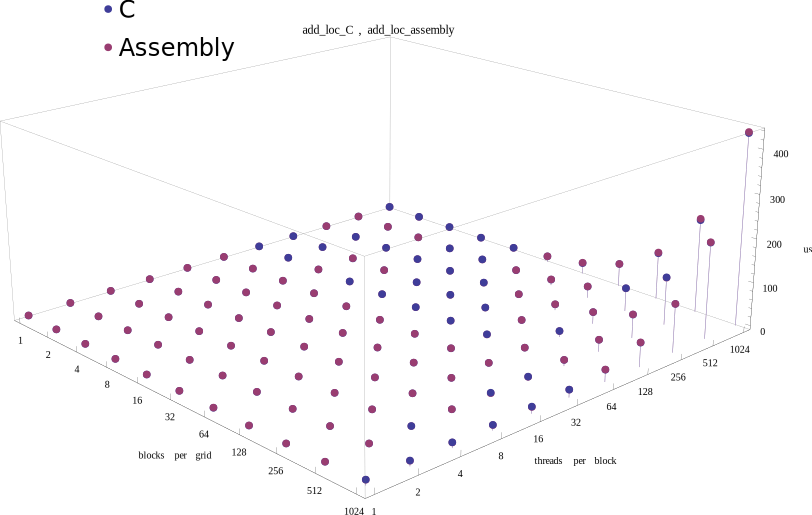
\includegraphics[scale=0.4]{figs/assembly_vs_c_loc_kepler_131_duration}
\caption{C vs. assembly 131-bit addition kernel execution time (local vectors)}
\label{fig:assembly_vs_c_loc_kepler_131_duration}
\end{figure}

As one can see, the difference between the 2 versions is negligable.
Figure~\ref{fig:assembly_vs_c_loc_kepler_131_registers} shows the difference in
register usage between the 2 versions.

\begin{figure}[h]
\centering
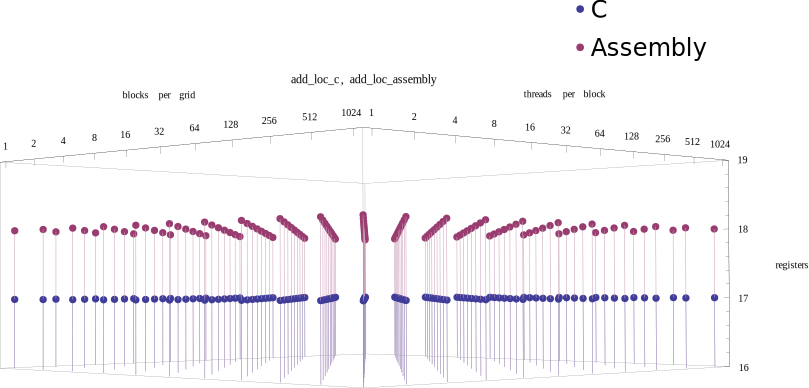
\includegraphics[scale=0.4]{figs/assembly_vs_c_loc_kepler_131_registers}
\caption{C vs. assembly 131-bit addition kernel register usage (local vectors)}
\label{fig:assembly_vs_c_loc_kepler_131_registers}
\end{figure}

\item C code would be more portable than our assembly statements.
It would also be safer to use, and much easier to debug (this project made us
learn this the hard way.)
\end{itemize}

\section{Project File Structure}
There are 2 main folders in our project, the \verb+scripts+ folder, which
contains all our python scripts, and the \verb+src+ folder, which contains all
the C code for actual testing on the GPUs.

\subsection{Scripts folder}
The \verb+script+ folder contains the following files:

\begin{description}
\item[\Q{constants.py}]
This is the central control point for the whole project, as it contains all the
constants used in the project, and influences the code that is generated.
An extract of the most important constants is given in
Listing~\ref{lst:constants.py_important_fields}, along with a short explanation.
Some of the constants defined in this file are needed by the C code, therefore
constants.py modifies all C files such that they contain all the up-to-date
values it contains.
An example of such a variable is \verb+min_bignum_number_of_words+.

\lstset{language=Python}
\lstset{caption={Important constants in constants.py},
        label={lst:constants.py_important_fields}}
\begin{lstlisting}
import math

precision = 239
bits_per_word = 32
blocks_per_grid = 1
threads_per_block = 1
file_name_operations_h = r'../src/operations.h'
number_of_bignums = threads_per_block * blocks_per_grid
min_bignum_number_of_words = math.ceil(precision/bits_per_word)
max_bignum_number_of_words = math.ceil((2*precision)/bits_per_word)

assert min_bignum_number_of_words == math.ceil((precision+1)/bits_per_word)
\end{lstlisting}

\begin{description}
\item[\Q{precision}] Precision the generated operations should support.
Any value is supported here, except all multiples of 32, for reasons specified
in section~\ref{sec:why_we_chose_assembly_over_c}.
This condition is asserted at the end of the file.
\item[\Q{threads_per_block}] Number of threads contained in a grid block.
Supported values are anything from 1 up to 1024, as our code failed to compile
for thread ranges that were any larger.
\item[\Q{blocks_per_grid}] Number of blocks contained in a grid.
Supported values are anything from 1 up to 1024, as our code failed to compile
for block ranges that were any larger.
\item[\Q{bits_per_word}] Primary data type of the device.
This field is useful if GPUs were to move from their current  32-bit primary
data type to a higher precision one.
It causes all the code generation algorithms to adapt accordingly.
\item[\Q{min_bignum_number_of_words}] This field represents the minimum number
of words that a bignum needs for its representation.
No bignum will ever use less storage place than this value.
\item[\Q{max_bignum_number_of_words}] This field represents the maximum number
of words that a bignum needs for its representation.
This value is used for storage requirements of the result a multiplication
yields.
No bignum will ever use more storage place than this value.
\item[\Q{number_of_bignums}] This field represents the total number of threads
that are being launched.
\item[\Q{file_name_operations_h}] This field tells the script which file it
should generate all the functions to.
\end{description}

\item[\Q{conversions.py}]
This file handles the conversions of numbers from Python's internal
unlimited-precision integer arithmetic to our GPU's number representation, which
is 2's complement notation.
The functions in this file are mostly used to verify that the results of our GPU
operations are correct.
Integers are kept as Python's basic signed integers, however, all binary and
hexadecimal values are kept as strings, as we have to transform them into two's
complement form.
Signed integers are converted to two's complement by getting their binary string
in signed and magnitude form.
If it is a positive number, then it is simply returned.
Otherwise, we apply the following forumla to get the representation of the
negative version of the number's absolute value (let's call it $B$):
$-B = \bar{B} + 1$.

\item[\Q{input_output.py}]
This file defines functions for writing bignums to a file in coalesced form, as
well as functions for reading coalesced bignums from a file, and reconstructing
their integer value from the two's complement representation.

\item[\Q{operation_checker.py}]
This file verifies if the bignums the GPU computed are correct.

\item[\Q{operation_generator.py}]
This is the main file of the project which generates our functions.
Note that the generated \emph{macros} are put in the file defined by
\verb+file_name_operations_h+ in \verb+constants.py+.

\item[\Q{random_number_generator.py}]
This file generates random numbers of the precision specified by
\verb+precision+ in \verb+constants.py+.
\end{description}

\subsection{Src folder}
The \verb+src+ folder contains the following files:

\begin{description}
\item[\Q{constants.h}]
This file is the central control point for the C part.
It contains some of the fields that were defined by \verb+constants.py+, which
are needed in order to know where to write results to, how much memory needs to
be allocated, \ldots
The important fields are listed below:

\begin{description}
\item[\Q{THREADS_PER_BLOCK}] Equivalent to \verb+threads_per_block+ in
\verb+constants.py+.
\item[\Q{BLOCKS_PER_GRID}] Equivalent to \verb+blocks_per_grid+ in
\verb+constants.py+.
\item[\Q{NUMBER_OF_BIGNUMS}] Equivalent to \verb+number_of_bignums+ in
\verb+constants.py+.
\end{description}

\item[\Q{bignum_types.h}]
This file contains the definitions \verb+MIN_BIGNUM_NUMBER_OF_WORDS+, and
\verb+MAX_BIGNUM_NUMBER_OF_WORDS+, which are respectively equivalent to
\verb+min_bignum_number_of_words+ and \verb+max_bignum_number_of_words+ defined
in \verb+constants.py+.
It also defines 2 important macros needed in order to know where a given bignum
is located in memory.
These macros are \verb+IDX(i, j, is_long_number)+ and \verb+COAL_IDX(i, j)+, and
are explained below:

\lstset{language=C++, label={}, caption={bignum\_types.h}}
\begin{lstlisting}
#define IDX(i, j, is_long_number) (((i) * ((is_long_number) ? (MAX_BIGNUM_NUMBER_OF_WORDS) : (MIN_BIGNUM_NUMBER_OF_WORDS))) + (j))
#define COAL_IDX(i, j) (((i) * (NUMBER_OF_BIGNUMS)) + (j))
\end{lstlisting}

\begin{description}
\item[\Q{IDX(i, j, is_long_number)}] This macro allows one to select bignums
from a \emph{non}-coalesced array.
Input \verb+i+ must satisfy
\verb+0 <= i < NUMBER_OF_BIGNUMS+, and chooses which bignum one wants to select.
Input \verb+is_long_number+ specifies if the bignums represented in the array
are bignums that are represented on \verb+MIN_BIGNUM_NUMBER_OF_WORDS+ words,
or \verb+MAX_BIGNUM_NUMBER_OF_WORDS+ words.
One needs to know if the data is a multiplication result, or just normal
bignums.
Input \verb+j+ must satisfy
\verb+0 <= j < MIN_BIGNUM_NUMBER_OF_WORDS+ or
\verb+0 <= j < MAX_BIGNUM_NUMBER_OF_WORDS+, depending on the value of
\verb+is_long_number+.
Input \verb+j+ allows one to select a particular word of a bignum.

\item[\Q{COAL_IDX(i, j)}] This macro allows one to select bignums from a
\emph{coalesced} array.
Input \verb+i+ must satisfy \verb+0 <= i < MIN_BIGNUM_NUMBER_OF_WORDS+, or
\verb+0 <= i < MAX_BIGNUM_NUMBER_OF_WORDS+, depending if the array is containing
multiplication results, or normal bignums.
Input \verb+j+ must satisfy \verb+0 <= j <= NUMBER_OF_BIGNUMS+.
Input \verb+i+ selects which element of a bignum must be accessed, and input
\verb+j+ selects which thread's bignum must be accessed.
Normally, one would use this in kernels when accessing coalesced global memory,
by looping over index \verb+i+, and using \verb+threadIdx.x+ as the value in
\verb+j+.
\end{description}

\item[\Q{benchmarks.cu}]
This file contains all our kernels, with which we launch our operation
benchmarks.
A benchmark consists of computing 10 instances of each operation one after the
other.
Every kernel reads its operands from the files \verb+random_number_generator.py+
created, performs the operation, then writes the results back to a file in
coalesced form for verification.
Each operation has 2 kernels, one that only uses coalesced global memory reads
for the 10 instances, and another which reads the operands to some local memory
before performing the operations.
This will be used so we can compare the latency difference between the 2
approaches.

\item[\Q{input_output.cpp}]
Contains functions to read coalesced bignum arrays from files, and to write
coalesced bignum arrays to files.

\item[\Q{main.cu}]
Selects which benchmarks have to be run.

\item[\Q{operations.h}]
Contains all the generated operations that have been created by
\verb+operation_generator.py+.
\end{description}

\section{Operations}
\subsection{Addition}
\subsection{Subtraction}
\subsection{Modular Addition}
\subsection{Modular Subtraction}
\subsection{Multiplication}
\subsection{Karatsuba Multiplication}

%
% --------------------------------------------------------------------------------
% Bibliography:
% -------------
% Internet:
% ---------
% http://en.wikipedia.org/wiki/Graphics_processing_unit
% http://en.wikipedia.org/wiki/Programmable_shader
% http://en.wikipedia.org/wiki/General-purpose_computing_on_graphics_processing_units
% http://en.wikipedia.org/wiki/Functional_completeness
% http://www.mathematik.uni-dortmund.de/~goeddeke/gpgpu/tutorial.html
% http://en.wikipedia.org/wiki/CUDA
% https://developer.nvidia.com/cuda-faq
% https://developer.nvidia.com/get-started-cuda-cc
% http://gmplib.org/
% http://en.wikipedia.org/wiki/Two%27s_complement
% http://en.wikipedia.org/wiki/Parallel_Thread_Execution
%
% Books:
% ------
%
% Papers:
% -------

\end{document}
